
\documentclass[conference]{IEEEtran}

%\usepackage{ifpdf}
\usepackage{float}  % For handling float environments like [H]
\usepackage{url}    % For handling URLs
\usepackage{multirow}
\usepackage{subcaption} % Required for subfigures
\usepackage{booktabs}
\usepackage{cite}
\pagestyle{plain}
\usepackage{amsmath}
\usepackage{float}
\usepackage{tikz}
\usetikzlibrary{shapes.geometric, arrows, positioning}%\usepackage{url}
\usepackage{placeins}


\ifCLASSINFOpdf
  \usepackage[pdftex]{graphicx}
  % declare the path(s) where your graphic files are
  % \DeclareGraphicsExtensions{.pdf,.jpeg,.png}
%\else
  % or other class option (dvipsone, dvipdf, if not using dvips). graphicx
  % and their extensions so you won't have to specify these with
  % every instance of \includegraphics
  % \DeclareGraphicsExtensions{.eps}
\fi
% graphicx was written by David Carlisle and Sebastian Rahtz.


% correct bad hyphenation here
\hyphenation{op-tical net-works semi-conduc-tor}


\begin{document}


\title{Recommender System}

% use a multiple column layout for up to three different
% affiliations
\author{\IEEEauthorblockN{\\ Hugo Veríssimo}
\IEEEauthorblockA{Foundations of Machine Learning 24/25\\
University of Aveiro\\
Aveiro, Portugal\\
hugoverissimo@ua.pt}
\and
\IEEEauthorblockN{\\ João Cardoso}
\IEEEauthorblockA{Foundations of Machine Learning 24/25\\
University of Aveiro\\
Aveiro, Portugal\\
joaopcardoso@ua.pt}}


% make the title area
\maketitle
\thispagestyle{plain}


% As a general rule, do not put math, special symbols or citations
% in the abstract
\begin{abstract}

\end{abstract}

\begin{quote}
\small
\noindent
\textbf{Keywords:} MovieLens, GroupLens, Recommender System, Collaborative Filtering
\end{quote}

\IEEEpeerreviewmaketitle


\section{Introduction}

Since the early 90's that the production rate of multimedia content has increased dramatically (pun intended). Initially, users relied mostly on video store owners, film critics on newspapers, friends. With increasing volumes of content, recommender systems have appeared as data-driven methods to reliably and quickly recommend movies based on the users' own appreciations.

% The use of similar datasets can help facilitate the comparison of RS, but it isn't the only way. Maybe add this further down the document, it is not so relevant in the introduction.

Recommender systems are information tools that provide users with recommended items (ideally) based on their list of preferences \cite{Konstan2012,KATARYA2017105}. These can be divided in different types, depending on the algorithm and approach to the data. Three categories can be considered: non-personalized, content-based, and collaborative filtering algorithms. Regardless of the algorithm of choice, these face crucial challenges: cold start problem (where it is difficult to tailor recommendations to a user without known preferences, or recommend an item with no reviews); data sparsity (given that most users review few items in the universe of possible items, leaving most of the user/item matrix empty); and scalability (as data grows exponentially, processing becomes evermore expensive and troublesome). These systems have been widely used in many different areas (online shopping, music, books, movie recommendation), and significant investment has gone into developing evermore personalized algorithms. A notable case for this was the Netflix prize competition in 2006, a moment where the research in the field skyrocketed. As a result, it was needed to develop better frameworks for comparison, considering not only the metrics, but data preprocessing, preparation, and routine, in order to ensure reproducibility across models and authors \cite{10.1145/2645710.2645746}.

For that reason, the developed recommender systems is based on one of the most widely used movie databases, MovieLens dataset, for education and development \cite{Harper2015}. The choice of this dataset allowed for a based comparison with algorithms from the literature, and facilitate the analysis and interpretation of the results here presented. 

\section{State of the Art}

The field of recommender systems is wide and covers many different algorithms and techniques. In the present work we focus on collaborative filtering using matrix factorization, as it is the main focus of the work here developed.

\section{Methodology}


\subsection{dados engenharia? tratamento?}

os dados contém 

100836 ratings, to 9724 movies by 610 users

contudo de modo a tornar o dataset um pouco menor e tp por nao querermos utilizadores novos, com poucas classificacoes de filmes, visto q qnd um utilizador tem poucas classificacoes ha uma metodologia diferente (vet ppts / literatura ?), foram removidos utilizadores com menos de 50 filmes avaliados e foram removidos filmes sem avaliacoes

pelo q ficamos com (9633 filmes, 385 users) e 93812 ratings no total

os dados foram separados em teste e treino, pelo que os ratings levaram split de 20\%, resultando em 75049 ratings para teste e 18763 para treino sendo o objetivo ver como a previsao dos ratings fica com os de treino



\subsection{dados análise}

\begin{figure}[H]
    \centering
    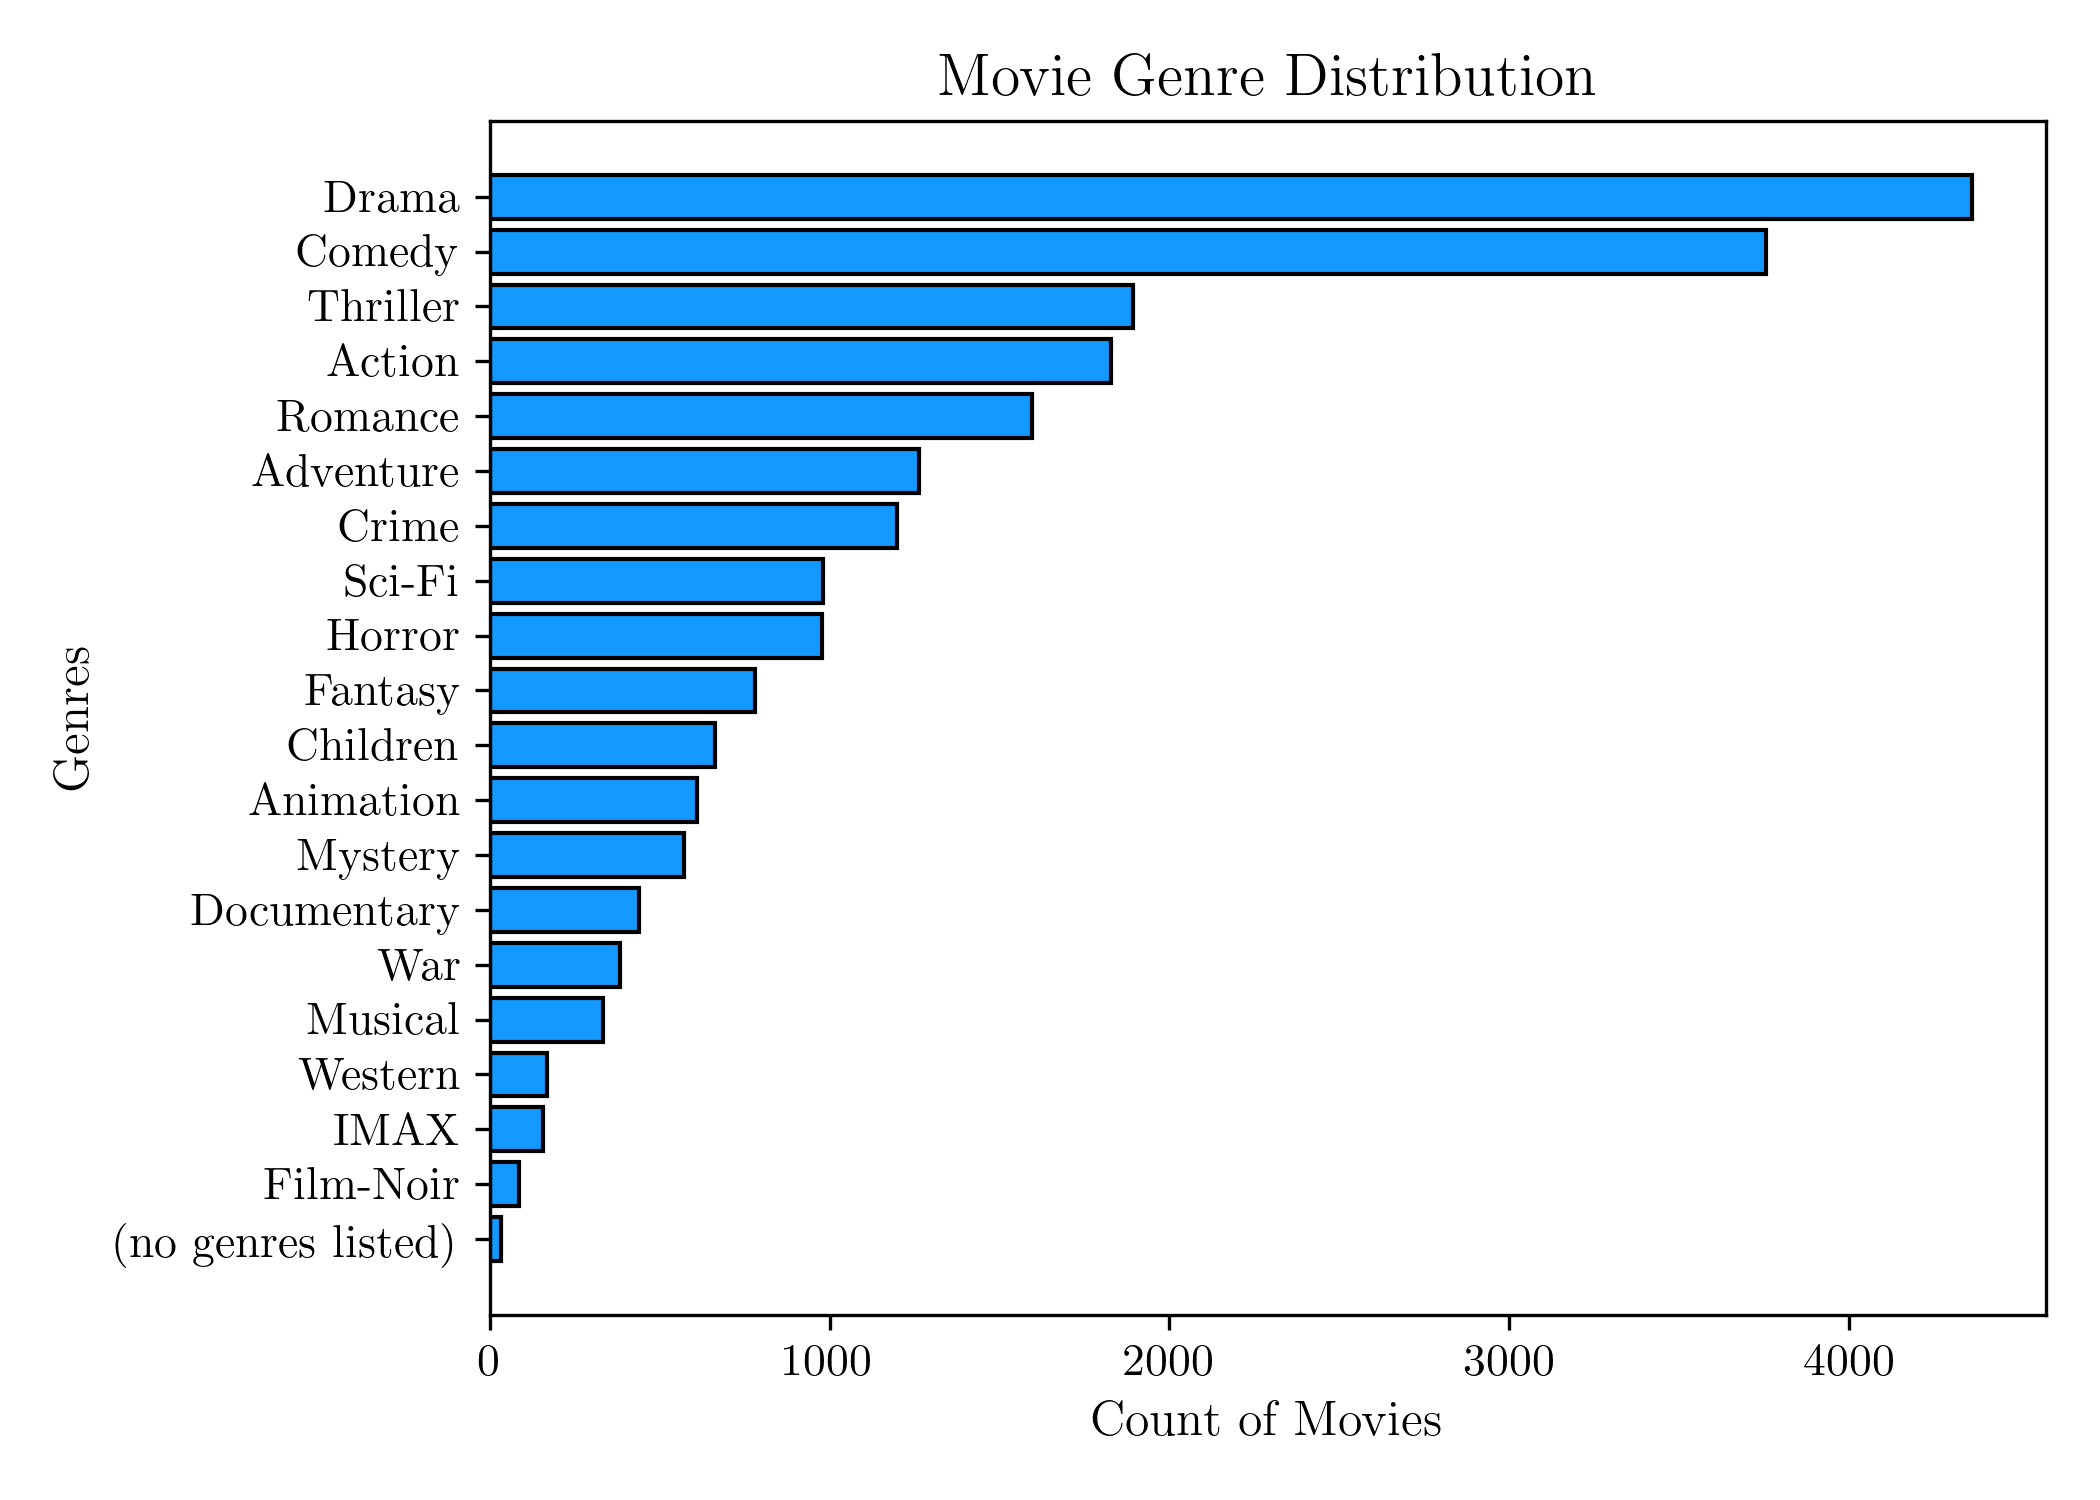
\includegraphics[width=1\linewidth]{assets/genre_distribution.png}
    \caption{CAPTIO CAPTION CAPTION}
    \label{fig:genre_distribution}
\end{figure}

\begin{figure}[H]
    \centering
    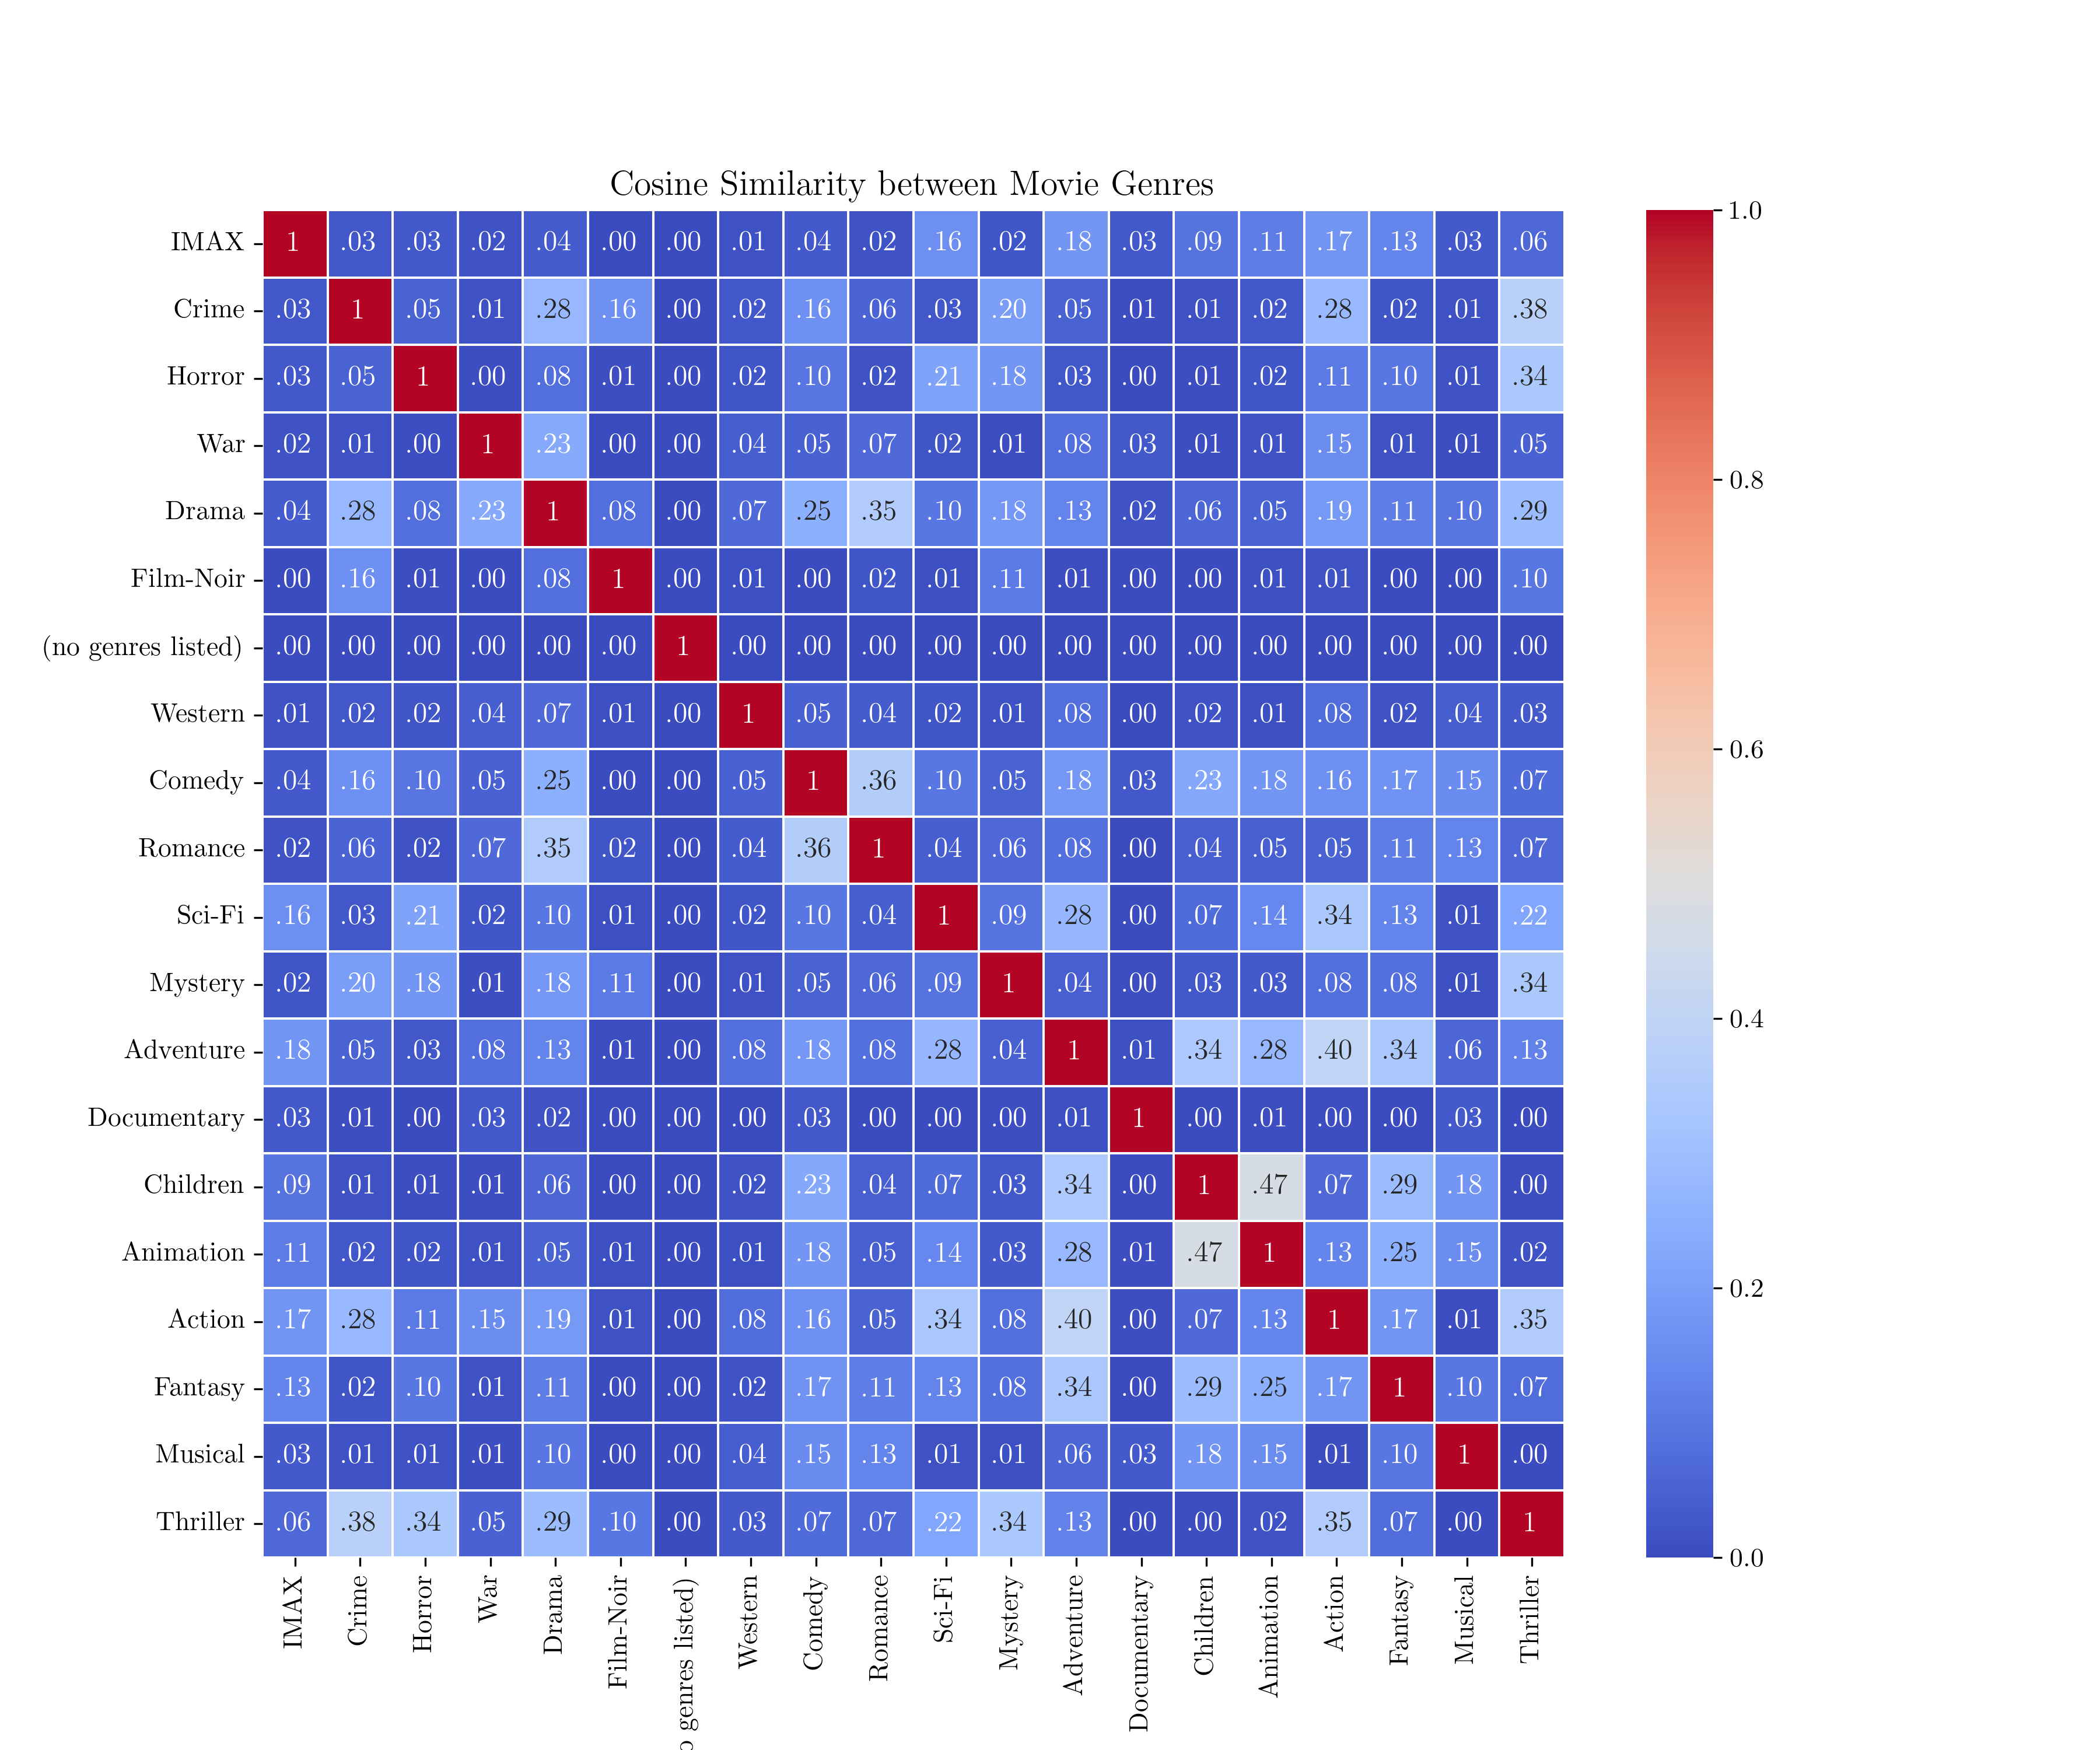
\includegraphics[width=1\linewidth]{assets/genre_similarity.png}
    \caption{CAPTIO CAPTION CAPTION}
    \label{fig:genre_similarity}
\end{figure}

na fig \ref{fig:genre_similarity} ve se relacoes como 

\begin{table}[H]
\centering
\caption{CAPTIO CAPTION CAPTION}
\label{tab:genre_similarity}
\begin{tabular}{llr}
\toprule
\textbf{genre} & \textbf{genre} & \textbf{sim} \\
\midrule
Animation & Children & .47 \\ 
Action & Adventure & .40 \\
Crime & Thriller & .38 \\
Romance & Comedy & .36 \\
Romance & Drama & .35 \\
\bottomrule
\end{tabular}
\end{table} 

\begin{figure}[H]
    \centering
    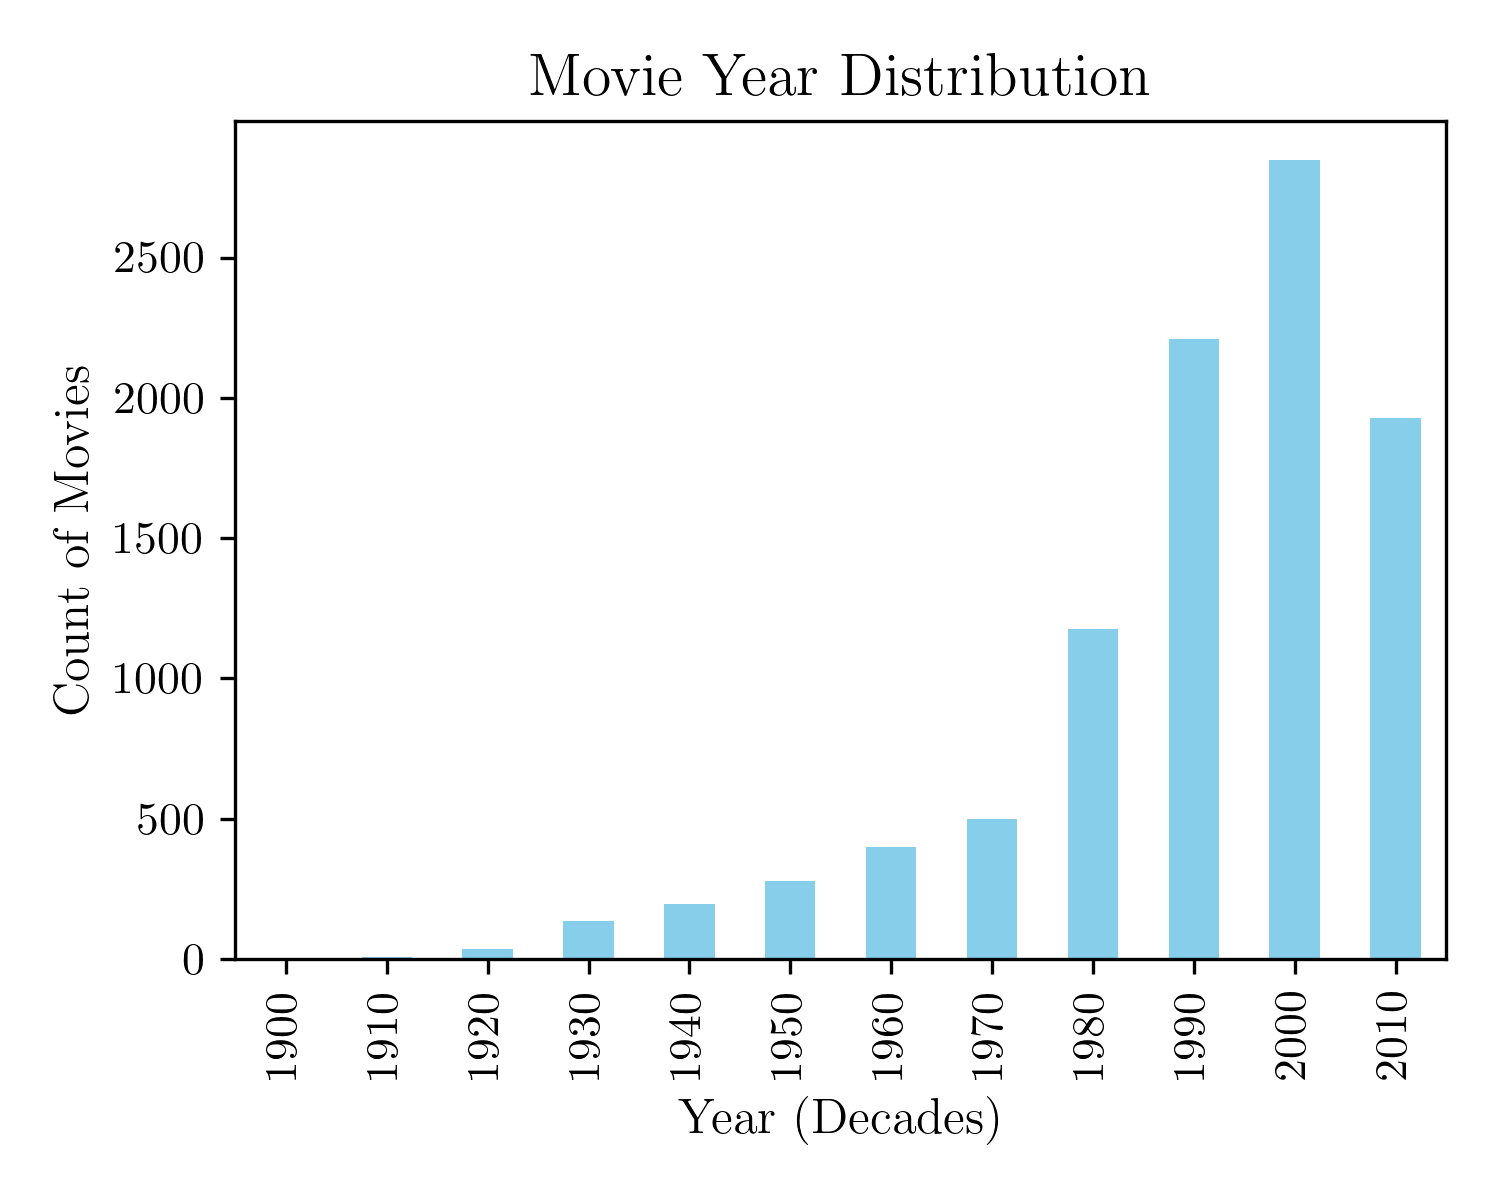
\includegraphics[width=1\linewidth]{assets/year_distribution.png}
    \caption{CAPTIO CAPTION CAPTION}
    \label{fig:year_distribution}
\end{figure}



\section{Classification Models}


\section{Logistic Regression}




\section{Discussion} \label{discussion_sec}
\subsection{Performance Metrics}


\subsection{Decision Boundaries}


\subsection{Literature Benchmark}


\section{Conclusion}


\section*{Work Load}

Both authors contributed equally to the project.


% trigger a \newpage just before the given reference
% number - used to balance the columns on the last page
% adjust value as needed - may need to be readjusted if
% the document is modified later
%\IEEEtriggeratref{8}
% The "triggered" command can be changed if desired:
%\IEEEtriggercmd{\enlargethispage{-5in}}


\bibliographystyle{IEEEtran}
\bibliography{references}

\end{document}



